% Course: AIM3
% Autors: Anil Pala, Franziska Adler
% Datum: 03.02.2015

\documentclass[a0,portrait]{a0poster}

\usepackage{anyfontsize}%for changing fontsize
\usepackage[ansinew]{inputenc}
\usepackage[T1]{fontenc}
\usepackage[english,ngerman]{babel}
\usepackage{amsmath} 
\usepackage{fancybox}
\usepackage{graphicx}
\unitlength1cm %picture environment 1 cm

%colums and boxes
\usepackage{multicol}
\setlength{\fboxrule}{1.5mm} %lines
\setlength{\fboxsep}{10mm} %margin text relation
\setlength{\columnsep}{15mm}     %colum space
\setlength{\columnseprule}{4pt}  % lines between columns

%page settings
\renewcommand\baselinestretch{1.2}
\parskip=0.5\baselineskip
\topmargin-30pt
\marginparwidth0mm
\oddsidemargin-20pt
\evensidemargin-20pt
\textwidth770mm
\textheight1140mm

% color
\usepackage{xcolor}
\usepackage{color} 
\definecolor{darkgreen}{rgb}{0,0.4,0.2} 
\definecolor{darkblue}{rgb}{0,0,0.5}
\definecolor{darkred}{rgb}{0.6,0,0.05}

\begin{document}
\pagecolor[rgb]{0.9,0.925,0.9}
% header
 \begin{center}
    {\huge \textbf{\\A Comparison of Online learning Na\"ive Bayes Classifier\\ on RSS Feeds using SPARK\\}}
 %   \vspace*{0.018\textheight}
  \end{center}
\begin{minipage}{0.4\textwidth}
\begin{flushleft} \large
\textbf{\emph{Authors:}\\
Anil \textsc{Pala} \& Franziska \textsc{Adler}}\\
%anil@pala.com \hspace{0.5cm} adler.franziska@gmx.de
\end{flushleft}
\end{minipage}
\hfill
\begin{minipage}{0.4\textwidth}
\begin{flushright} \large
\textbf{\textsc{\color{darkred} \Large TU Berlin}\\
Advanced Information Management III\\
Scalable Data Analytics and Data Mining}
\end{flushright}
\end{minipage}
\newcommand{\HRule}{\rule[-10mm]{805mm}{1mm}} \HRule \\[0.5cm] %line

%create first Box
\fcolorbox{darkgreen}{white}{\parbox{\textwidth}{%

    \begin{multicols}{2}      
      \begin{center} \textbf{\huge Motivation \& Problem Statement} \end{center}
Many practical applications rely on immediate data. The need for solutions to continuously conduct analyses as mathematical computations on large data amounts led to new technologies in the past years. Stream processing operates on real-time data for example through stream windowing and analytical operations within those. Since data distributions might not remain static over time a precomputed (batch) model for analysis can produce poorly results after some time [1]. The reconstruction or updating of the underlying analytical model to receive accurate results is required. This problem is known as Concept Drift. In this project we are using unstructured streaming data from BBC RSS feeds in order to classify them to their corresponding category. We focus on the evaluation of a Na\"ive Bayes Classifier with different model-update approaches to compare their analytical performance according to Concept Drift. 

    \end{multicols}}}

\vspace{0.8cm}
%create second Box
\fcolorbox{darkgreen}{white}{\parbox{0.4775 \textwidth}{%
      \begin{center} \textbf{\huge Data \& Setup} \end{center}
For our evaluation purposes of classifing streamed textdata we are using RSS feeds from BCC. A RSS feed is a collection of tags in xml structure which contains tags for title, a description and an url among other tags. Those listed are used in our applicaton. Our data points are constructed from title and description of the feed, the url gives us the respective label.\\
setup   


}}
\hspace{0.8cm}
%create 3. Box
\fcolorbox{darkgreen}{white}{\parbox{0.4775 \textwidth}{%
      \begin{center} \textbf{\huge Streaming} \end{center}
In order to deal with the continuos nature of the data, traditional programming primitives are not of much help. In order to make programmers's job easier, libraries providing higher lever abstractions are introduced. Knowing that, for a news feed classifier we need to split the 'main' stream into multiple streams to treat different portions of stream differently. For example, there needs to be at least two channels of streams branching out from the main one having the test items and training items. The main flow of the streaming logic we used is depicted in the figure.[2]\\
\begin{center}
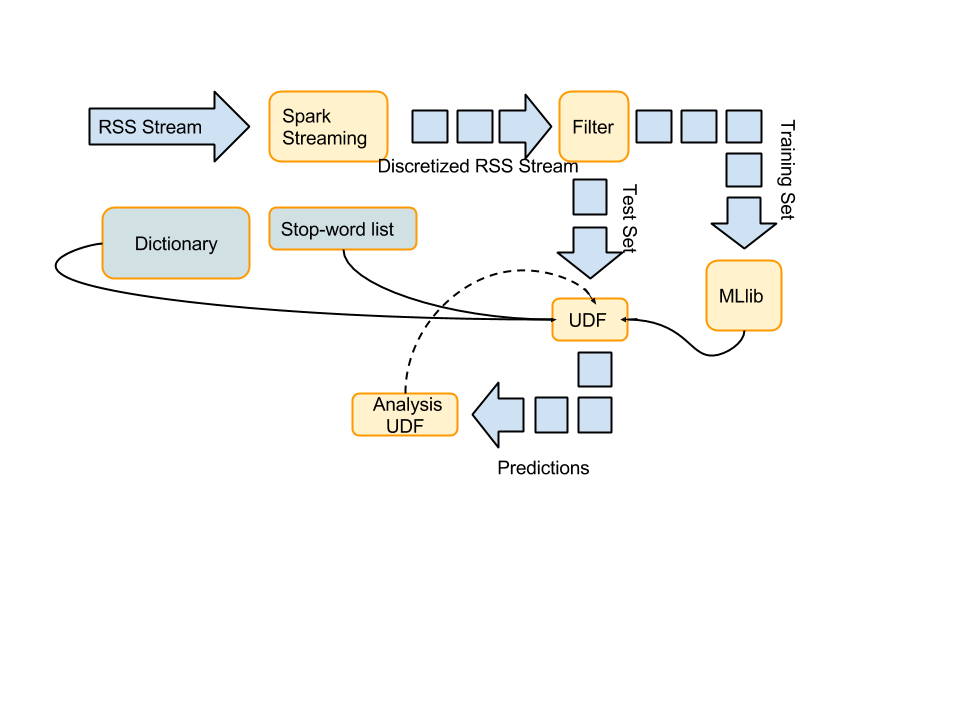
\includegraphics[width=0.2\textwidth]{./time_models/streaming_diagram}
\end{center}
}}
\hspace{0.8cm}


\vspace{0.8cm}
%create 4. Box
\fcolorbox{darkgreen}{white}{\parbox{\textwidth}{%

    \begin{multicols}{4}      
      \begin{center} \textbf{\huge Methodology} \end{center}
\textbf{\large Batch and On-line}\\
The batch model implements a classic Traing-Testing-Phase setup. A subset training points are pre-collected from a stream and used to build a final model on  which three testsets are applied. The batch model functions as a reference model to observe the performance of the initial training over time. \\
\textbf{\large Bruteforce}\\
On the other hand On-line Learning will change the model with the arriving of new data points.
The bruteforce approach updates the model after a period of time through retraining. Based on a sliding window over the stream with a constant number of data points 
the model is rebuilt.\\
\textbf{\large Threshold-triggered}\\
As a variation of the bruteforce model-update the threshold triggered one will rebuild the model on a sliding window as soon as the performance of our model is beneth a certain threshold. \\
\textbf{\large Incremental}\\
The incremental model updates the models properties with new arriving data points. \color{red}TODO TODO TODO TODOTODO TODOTODO TODOTODO TODOTODO TODOTODO TODOTODO TODOTODO TODOTODO TODOTODO TODOTODO TODOTODO TODO
 %changed to Methodology
    \end{multicols}}}

\vspace{0.8cm}
%create 5. Box: BATCH----------------------------------------------------------------------------------------
\fcolorbox{darkgreen}{white}{\parbox{0.24 \textwidth}{%
\textbf{Batch}\\

For Offline learing the model was built within the first three days out of 600 data points. The following four days with 1248 data points created the first test set for this model. A second and a third test set where created after the previous testphase and contained 1102 and 1172 data points, respectivly RSS feeds.\\

      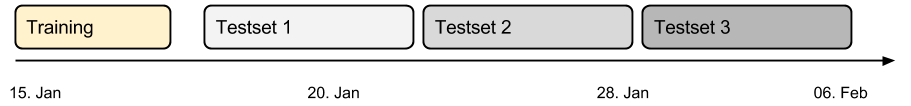
\includegraphics[width=0.24\textwidth]{./OfflineModel.png}\\
}}
\hspace{0.8cm}
%create 6. Box: Bruteforce and Errortriggered ----------------------------------------------------------------
\fcolorbox{darkgreen}{white}{\parbox{0.4775 \textwidth}{%
    \begin{multicols}{2}    
\textbf{Bruteforce and Error-triggered}\\

The window size for the bruteforce model contains 600 data points. After 400 test points we led it retrain with the last 600 data points. We then waited for 1000 data points and second retrain phase followed which was tested also with 1000 new data points.\\

   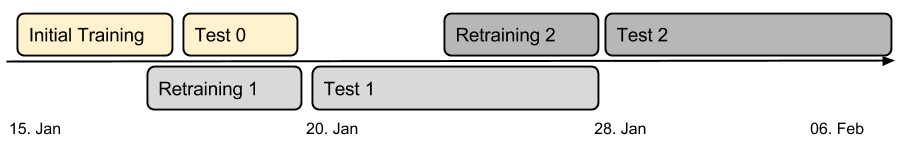
\includegraphics[width=0.2\textwidth]{./BruteforceModel}\\
The window size of the error-triggered model is constructed like the bruteforce update out of 600 datapoints. Due to our observations an diserable accurency threshold of 63\% seamed reasonable. A sanity window of testpoints ensures that at least 300 new data points arrive and based on their performance the model is rebuild or not.\\

   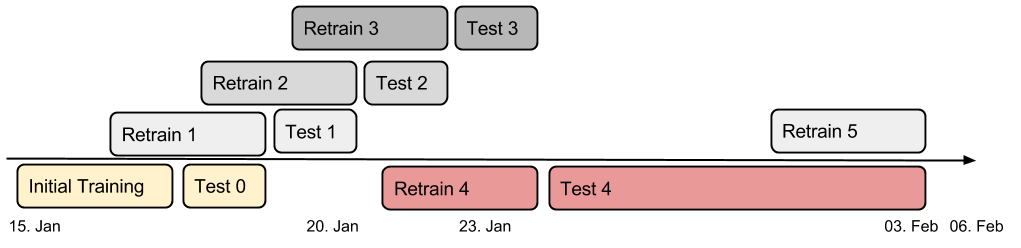
\includegraphics[width=0.2\textwidth]{./Errortriggered}
\end{multicols}}}
\hspace{0.8cm}
\fcolorbox{darkgreen}{white}{\parbox{0.18 \textwidth}{%
\textbf{Incremental updates}\\


 
}}

%create 7. Box: Results --------------------------------------------------------------------------------------
\fcolorbox{darkgreen}{white}{\parbox{\textwidth}{%
The offline versions result with 1000 test points per intervall is always around 60\% even though it decreased at the last testing phase. 
The offline versions result with 1000 test points per intervall is always around 60\% even though it decreased at the last testing phase. The offline versions result with 1000 test points per intervall is always around 60\% even though it decreased at the last testing phase. The offline versions result with 1000 test points per intervall is always around 60\% even though it decreased at the last testing phase. The offline versions result with 1000 test points per intervall is always around 60\% even though it decreased at the last testing phase. The offline versions result with 1000 test points per intervall is always around 60\% even though it decreased at the last testing phase. 
   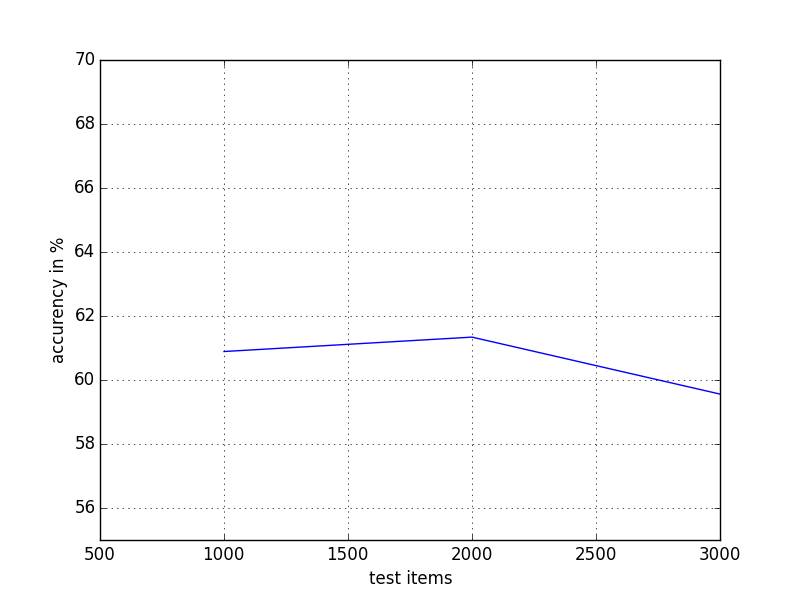
\includegraphics[width=0.2\textwidth]{./batchPlot.png}\\

The bruteforce model which updates after 
   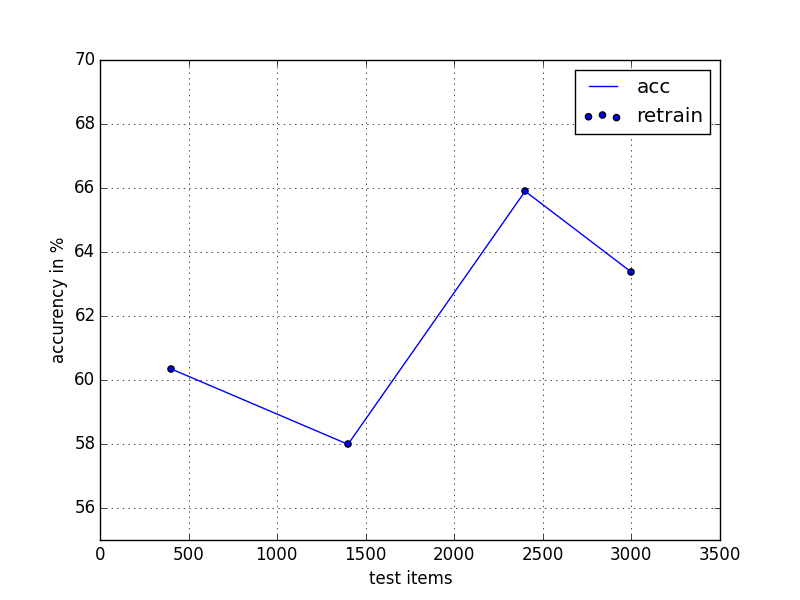
\includegraphics[width=0.2\textwidth]{./bruteforcePlot.png}
   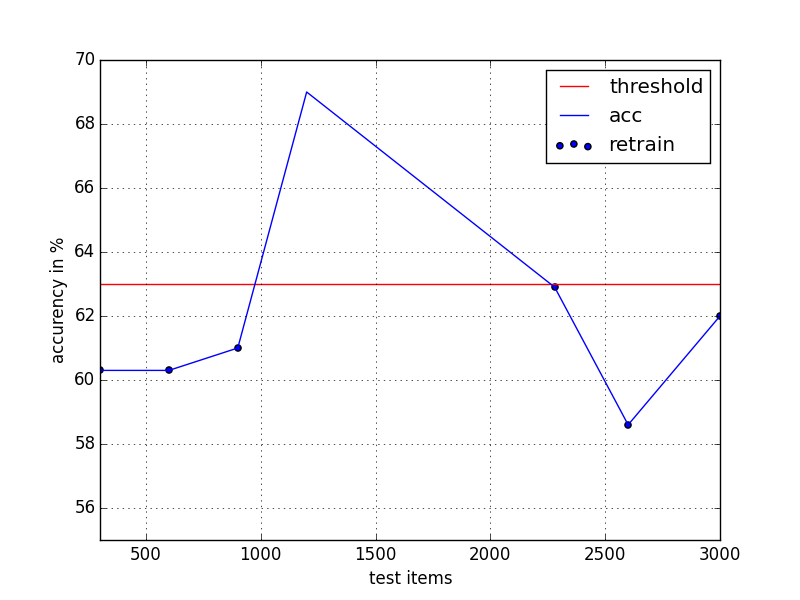
\includegraphics[width=0.2\textwidth]{./errortriggeredPlot}
   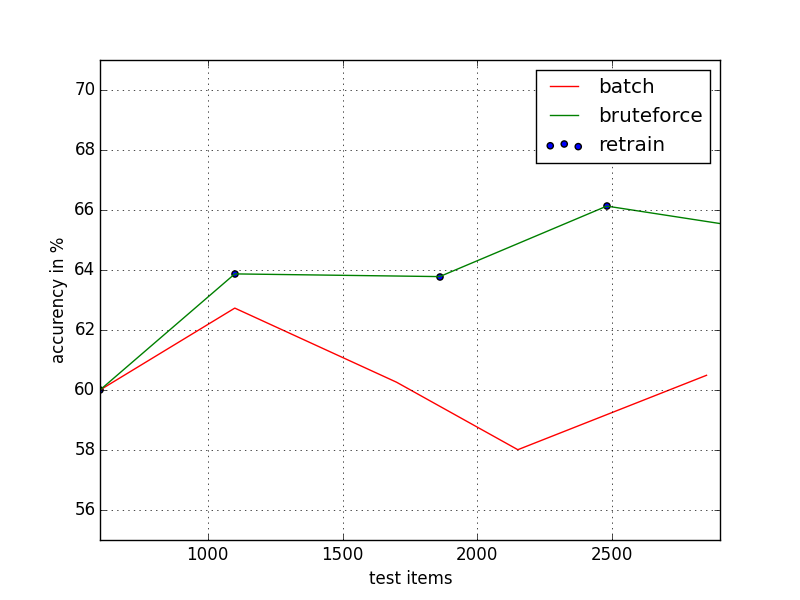
\includegraphics[width=0.2\textwidth]{./batchVsbruteforce}
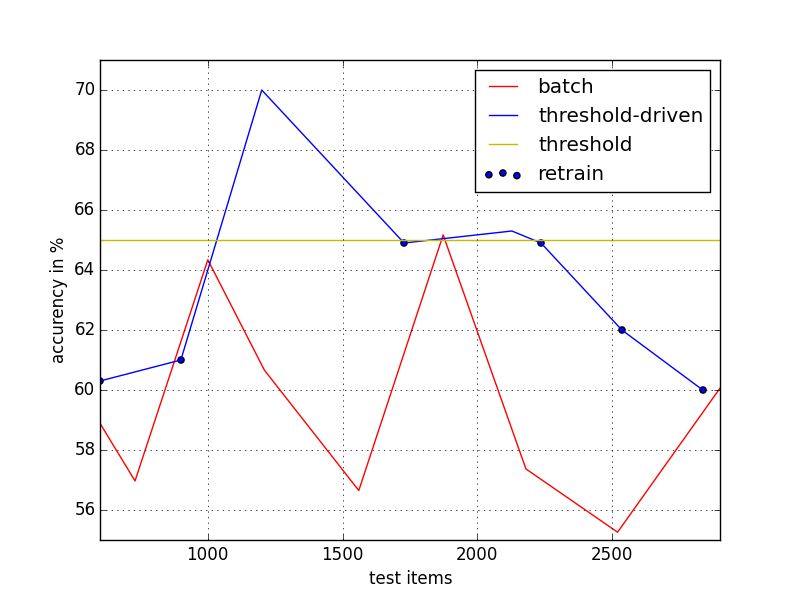
\includegraphics[width=0.2\textwidth]{./batchVSerror}\\
}}

\vspace{0.8cm}
%Literature
\fcolorbox{darkgreen}{white}{\parbox{ \textwidth}{%
      \renewcommand{\baselinestretch}{1.05}\small\normalsize
\begin{thebibliography}{9} 
%\begin{left} \textbf{\huge Literature} \end{left}
\bibitem{zitat1} \textsc{C\'esar A. Astudillo and Javier I. Gonzalez}\textit{Concept Drift Detection Using Online Bayesian Classifier},Proceedings of the XXXII International Conference of The Chilean Computer Science Society, 2013.
\bibitem{zitat2} \textsc{Zaharia, Matei and Das, Tathagata and Li, Haoyuan and Shenker, Scott and Stoica, Ion}, \textit{Discretized Streams: An Efficient and Fault-tolerant Model for Stream Processing on Large Clusters}, Proceedings of the 4th USENIX Conference on Hot Topics in Cloud Computing, 2012.
\end{thebibliography}



}}
\end{document}